\chapter{Related Work}

The TTS conversion is not a new field and people have been working on this field before electronic
signal processing techniques. In beginning, people tried to build machines which were used to
create human sound. After the development of computers, better systems were built using different
techniques. In \cite{swetha2013text}, basic speech synthesizing technique are discussed 
which works by concatenation of small recorded speech segments called phonemes to form
complete speech. Each word is first divided into syllables and then corresponding voice signal for each syllable
is concatenated in order to get pronunciation for whole word. This concatenated word has some
delay between pronunciations of each syllable which is removed and as a result of which final
pronunciation of that word is obtained. Problems like Text Preprocessing, Pronunciation and
Prosody makes it difficult. In Text Preprocessing, digits and abbreviations are converted to full
words. Other problem is guessing correct pronunciation of a word. For example, word “lives” has
different pronunciation in “He lives in Lahore” and “He saved two lives”. To create naturalness in
sound, stress and intonation are applied to the input text which is also a very complex task.

Two sub parts of text-to-speech system Text analysis and word pronunciation were discussed in \cite{liberman1992text}. 
TTS system is divied in 4 sub parts: text analysis, word pronunciation, phonetic interpretation and signal
generation. Text analysis step included division of text into sentences, words, phrases and expansion of abbreviations etc.
two main reason for text analysis were given on is use of letters in words in different contexts, and the other reason is its use
in pitch and amplitude modulating. In text analysis, sentence division and part of speech tagging is done by using heuristic solutions \cite{riley1989some}
and dynamic programming respectively. For word pronunciation, hybrid natured approach was used in which dictionary method is used for about 99.9\%
words and for only 0.1\% words which are mostly unstressed syllables, letter to sound rules were followed. 

A technique based on letter to sound rules is also developed in \cite{elovitz1976automatic}. Total 329 letters to sound rules have
been created. These rules take text as input and translate it into phonetic alphabet which in turn converted to synthetic sound.
This system produces about 97\% correct pronunciation of phonemes. The paper also describes software and hardware
requirement and overall performance statistics of this system. The dataset is developed by extracting
50,000 words from standard Corpus, Corpus of Present-Day Edited American English i.e. Brown
corpus \cite{ku1967computational}. The system gave accuracy of about 93\%. A more
improved system was proposed in \cite{carlson1982multi} and \cite{klatt1982klattalk}. 
In \cite{klatt1982klattalk}, a TTS system is developed for English and simple numerical and algebraic expressions. 
The system is rule based system having 500 letters to sound rules. However, it can use pronunciation dictionary of 1500 words for exceptions. 
The system interface provides facility of selection of voice types (Male or Female). The word boundaries and probable
position of phrases and clauses is analyzed by syntactic analyzer. The phoneme of words are then passed to synthetic speech
synthesizer that convert phoneme to sounds by following extensive set of rules and rules for consonant-vowel transitions. 
TTS system is divided in two sub processes, text analysis (conversion of text to
corresponding linguistic representation that comprises of phoneme, stress and boundaries and positions of respective vowel
or consonant and durational phenomena such as pauses, interaction between segments \cite{klatt1979synthesis} and other one is
speech synthesis in which sequence of phoneme are converted to speech sound by following set of rules. The input data is
preprocessed, the words which are abbreviations are converted to their text and if dictionary does not have their respective
words the abbreviation is pronounced as word. After preprocessing the words are exposed to letter to sound rules, 500 rules
were formulated, the rules are formulated by considering linguistic principles. If an unstressed function appear in text and
there is no rule for it then it is passed to pronunciation dictionary. The results show that about 95\% rules were successful
when executed. The syntactic analyzer then determines the structure of sentence according to its pauses and boundaries. The phoneme to speech rules
are divided into two components phonological that provide information of stress, rhythm and duration of words in a sentence.
All these outputs are then passed to synthesizer that produces synthetic sound. Synthesizer is simple version of \cite{klatt1980software}.


In \cite{carlson1982multi}, a text to speech system is presented which require some hardware resources as well with the enhancements in microprocessor, 
memory and signal processor technology. This TTS system can be put into portable form and can be used anywhere with different systems. A higher level language is
developed in laboratory that can be easily used for linguistic processes. These enhancements and developments in hardware
and software level made transforming of text to speech at 250 wpm rate. This combination of hardware and software is tested
against several applications used for handicaps. The main purpose of this system is to make a framework that will
be used for conversion of any language text to speech. A TTS system for Azerbhaijani language is developed using concatenative
synthesis in \cite{aida2010main} where small recordings were concatenated to make speech waveform.

In \cite{huang1996whistler}, Whistler which is a Text-to-Speech engine developed by using prosody and
concatenative speech parameters that were extracted through use of probabilistic learning methods. Whistler engine produce
speech which appears to be very much real. This system can also help to build TTS system for other languages.

A formant and concatenative synthesis is developed in \cite{huang1997recent}
where small segments of phonemes were concatenated to form whole speech. A training database was used contains about 6,000 phonetically balanced sentences recorded in natural style. The technologies used in whistler can considerably facilitate the
process of creating generic TTS system for new speech style. This engine supports MS Speech and requires less than 3 MB memory.

In \cite{hunt1996unit}, linear regression and unit selection 
based speech synthesis is designed using ATR Japanese database. In this algorithm, raw text is converted to phonetic strings and against each phoneme, best candidate unit from a huge database of speech units is selected with \textit{Viterbi} search. By concatenating these units, target waveform is generated. The units in database can be considered as state transition network where each unit represents a different state. The cost of the system depends on target cost and cost of the concatenation of units. The each phoneme and unit is represented by a multi-dimensional feature vector. The target cost is measured by the weighted difference of target and candidate feature vector. Similarly concatenation cost is also weighted sum of sub-cost of concatenation. Cost function can be trained in two different ways. In Weight Space Search method, units are searched with \textit{Viterbi} and distance between constructed waveform and
natural waveform is minimized. In Regression Training, linear regression is used to choose best unit from list of all possible
units for a given phoneme. 

Statistical parametric speech synthesis is another approach which uses parameters to describe
speech \cite{king2010beginners}. This technique works better than
concatenative technique on smaller data. On larger data, concatenative synthesis can produce better quality speech. In this technique, Hidden Markov model (HMM) or model firmly related to HMM are used for training model over given data. Hidden Markov model (HMM) based statistical parametric speech synthesis has gained popularity because of its ability to produces high quality speech automatically with parametric flexibility and less data and resources \cite{black2007statistical}.

A multi-dimensional Gaussian distribution based Hidden Markov model based statistical parametric speech synthesis system was developed in
\cite{yoshimura1998duration}.  In this technique, decision tree based context clustering is used for duration models clustering. The contextual factors are also considered with phone identity factors. Mel-cepstral coefficients are
calculated and model is trained by these coefficients. State of the context dependent HMMs is clustered using decision tree based
context clustering technique \cite{odellj.j1995}. In state duration modeling, multi-dimensional Gaussian distributions are
used to model Hidden Markov model. After estimation of duration models, using decision tree based clustering techniques,
they are clustered. By traversing decision tree, all contexts can be searched. Contextual factors which effects timing of
events in speech are also taken into account and resultant speech shows that it has good quality and natural timing. For testing
of system, 450 sentences of Japanese are used for training of system. Sampling of speech signal is done at 16 kHz. Feature
vector is composed of 25 mel-cepstral coefficients. There were 3030 states and 2984 distributions in output of the system.
The listening tests show that synthesized speech has good quality and it has natural timing even if speaking rate is changed to
some degree.

A similar system is designed in \cite{tokuda2000speech} using Hidden Markov Model and evaluated it by taking input
from Japanese database and by generating feature vector of those sentences and compared with
original speech. The parameters in this system are generated with Hidden
Markov model. The state sequence fully or partially is hidden due to which iterations are performed for parameter generation and
forward-backward algorithm is used for the situation where state sequence is provided. This algorithm, from multi-mixture HMMs,
can generate clear formant structure.

A Hidden Markov model and unit selection based system is proposed in \cite{tokuda2002hmm} in which model is trained with speech database and excitation and spectral parameters are extracted. These parameters are modeled by context dependent HMMs. To find
accurate model parameters, decision tree based context clustering is used. The parameters are then used to generate speech
signals. These parameters can be used to control speech characteristics. In \cite{harashima2006review}, Hidden Markov model and rule based approach is applied 
on voices taken from e-learning courses and online lessons for dataset creation and tested by
generating voices and given as input to students to interpret it.

Corpus based approach for Expressive Prosody Modeling is applied in \cite{eide2004corpus} where 
manually produced dataset was used. To evaluate the synthesized
speech, the output is given for testing to 32 native English speakers. For bad news, good news and
for yes/no the accuracy is 70.2\%, 80.3\% and 84\% respectively.

% Tones and Break Indices ToBI are discussed on American English in \cite{pitrelli2004tobi}. Majorly
% bi-gram and tri-gram were used to predict the occurrences of particular word or letter. Analysis
% was performed by multiple techniques. The corpus was divided into following five yes-no
% questions, either-or questions, other questions (hereafter, “wh-questions”), exclamations, and other
% declarative sentences categories for the analysis purpose. Analysis by word frequency count
% produced not good results and the reason was that the data was of variant types. The results show
% that professional speakers produces better and informative prosodic events as compared to
% ordinary speakers.

Hidden Markov model based approach is used in \cite{baloyi2012text} to construct
speech synthesizer for Xitsonga which is an African language. The dataset used here consists of phone
set of consonants and vowels and by using these sets, set of letter to sound rules is also prepared to be used in speech synthesis system. The main tool used for speech synthesis is HTS toolkit \cite{hts_2.2} with other software that support to setup complete environment for text-to-speech conversion.
The technique used in this study is HMM because the statistical parametric speech synthesis based on Hidden Markov model
can be used to synthesize speech waveform with requiring huge dataset for training. The system received acceptability
of 92.3\%. 

TTS system for Fon language is designed in \cite{dagba2014text} using Multisyn algorithm \cite{clark2007multisyn}
which consists of Natural Language Processing (NLP) and Digital Signal Processing (DSP)
modules. NLP consists of segmentation, Letter-to-Sound conversion and back-off rules module.
Back-off rules are applied when input text contains some characters that are not in us know
characters. DSP module than choose required unit from database of units are concatenate them to
form complete speech signals.

In \cite{ganai2016text}, hybrid text to speech converter is developed by
concatenating benefits of HMM based TTS system and waveform based TTS system. For developing it, an audio phoneme library is used. The main
edge of developed system over other is that it produced more human like voice/speech. The experiments were took in
matlab and a phoneme library is developed that consists of audio files and dictionary of words with their phoneme. Sentence is
taken as input then model parsed it into words. The system analyze each word get its phoneme and combine all phonemes
and plays the sound. Waveform for each sound is also presented. This sub-ban speech synthesized approach is obtained by
this combination of models that improved the quality of synthesized speech. The current model is not good enough, in future
system will be improved to get better controls.

In \cite{merritt2013investigating}, author discussed shortcomings of Hidden Markov model and majorly focused on the findings that HMM based TTS system are not better than simple concatenative TTS systems. Experiments performed and then through pairwise listening test the HMM based system evaluated. Based on the responses of qualities, model molded to tackle further situational problems. In figure \ref{fig:Merritt_tts}, architecture of this system is shown.
\begin{center}
	\begin{figure}[hbtp]
		\centering
		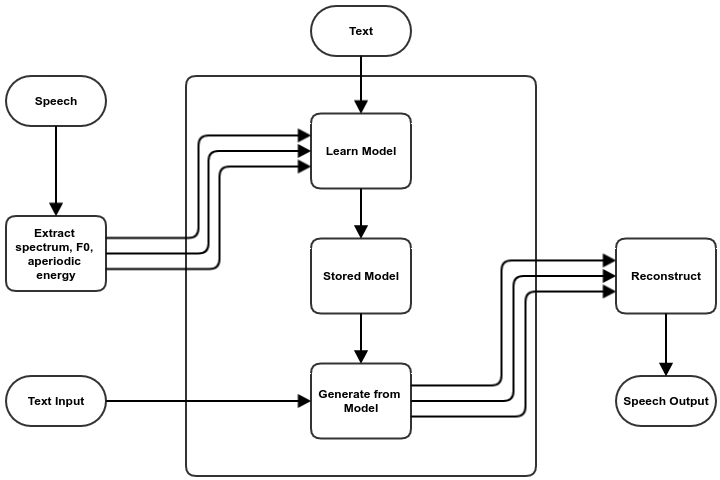
\includegraphics[width=\linewidth]{images/Merritt_tts.png}
		\caption{TTS System Architecture using HMM speech synthesiser}
		\label{fig:Merritt_tts}
	\end{figure}
\end{center}

Experiments show that this is secondary problem. When variance is too high then smoothing has a beneficial effect as it
reduces the variance and bring the points closer to the natural one. For future, needs to work over spectral envelope over-smoothness, averaging across multiple tokens of similar speech sounds, model boundary discontinuities in the trajectory and
inconsistencies between the different speech parameter streams \cite{merritt2013investigating}.

A more advance technique is Neural Network based technique as it works better than Hidden
Markov model based technique. Time domain neural networks with
database containing sounds of words called phonemes is used in \cite{karaali1998text}. The basic flow of the system involves
speech recording, speech labelling, voice coder and input processing using Time Delay Neural
Network. The figure \ref{fig:Time Domain Neural Network based TTS System} shows the block diagram of system.

\begin{center}
	\begin{figure}[hbtp]
		\centering
		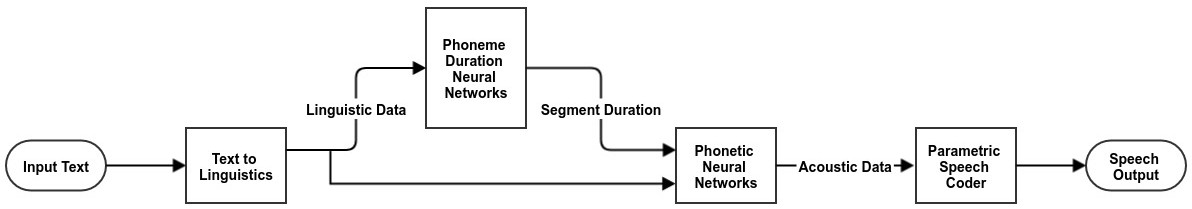
\includegraphics[width=\linewidth]{images/time_domain_neural_network.jpg}
		\caption{Time Domain Neural Network based TTS System}
		\label{fig:Time Domain Neural Network based TTS System}
	\end{figure}
		
\end{center}
Neural network based techniques are used to learn features automatically during training along with the combination of various techniques 
like linear regression and neural network in \cite{yoshimura2016hierarchical}. Dataset of all previous Blizard Challenges \cite{blizzard_2009_corpus} and
afterwards up to 2013 were used. Model was evaluated using 5-fold cross validation. The given model gave 0.11\% and 0.17\% error for LR+LR and LR+NN 
respectively.

Deep Neural Networks is applied in place of Hidden Markov model in \cite{ze2013statistical} as HMM
based system cannot model complicated context dependencies. Deep Neural Networks (DNN) can
cover limitations in HMM based system and can also outperform HMM based system. 

Recurrent Neural Networks (RNN) is applied in \cite{fan2014tts} by using the Bidirectional Long
Short Term Memory (BLSTM) with dataset consisting of 5000 training utterances and 200
utterances for testing the system. Whole recording was done in voice of female native speaker.
Objective and subjective evaluation measures are used to find distortion between natural and
synthesized speech and quality respectively. The preference results that hybrid system is better as
hybrid gave 44\%, 59\% and 55\% accuracy whereas neural network, HMM and DNN gave 29\%,
22\% and 20\% accuracy respectively. In \cite{muthukumar2016recurrent} Recurrent Neural Network (RNN) postfilters 
are used for speech synthesis. 

Neural Networks is used in \cite{wu2016merlin} with dataset consisting of 328 hours was collected in
voice of native 1506 speakers. The model is tested by giving 20 sets of randomly selected from
evaluation set and asked them to rate output of each set between 0 and 100.

Natural Language Processing unit is very importing unit in speech synthesis system as it handle all language related issues.
This unit performs a list of steps for its complete operation which contains tokenization, semantic tagging, string generation,
syllabification, stress and intonation marking etc. 

\cite{saleem2002urdu} and \cite{urdu_text_preprocessing} discuss such unit for Urdu language. This unit is divided in two parts called as preprocessing and phonological processing unit. Pre-processing unit converts number, date and time into their respective literal strings. For example, 100 and 5-11-2002 will be converted into \texturdu{سو} and \texturdu{پانچ نومبر دو ہزار دو} respectively. Special symbols like \$ and & are also handled in pre-processing unit. Last stage of pre-processing unit is grapheme into phoneme convertor. Phonological processing unit contains syllable marker which marks syllable boundaries and stress and
intonation markers mark stress and intonation. A speech corpus is developed using 10 hours recorded speech of professional speaker containing of 1036 sentences in \cite{mumtaz2016break}. Globalphone which is a database of multilingual types is elaborated in \cite{schultz2002globalphone}. This
database contains high quality voice vocabulary which can be used for voice recognition and text to speech system. It
contains dataset of consisting more than 300 hours in voice of 1500 native speakers. It mainly cover English, Arabic,
Japanese, Turkish and 11 more languages. Scientific work done on Urdu language is limited mainly due to the reason that
there is not enough material related to phonetic strings are available for Urdu. 

In \cite{urdu_tts_db_kashif2015}, Neural Networks consists of feed forward network, back propagation for weight updation is used to generate 
speech synthesis system for Urdu. An interface is designed and tested. Mean Square Error of designed system is used as performance parameter. 
The MSE is 0.00867 of proposed system. A large database consists of 59 Urdu characters, vowels and numbers is created for this system. The designed model only
produces synthetic sound of single character. In future, urdu sentences are added to generate output in the form of full text.

In \cite{saleem2002urdu} consonantal and vocalic sounds for Urdu Language is discussed . Bi-Lingual Text to Speech Synthesis 
System for Urdu and Sindhi is designed in \cite{shah2004bi} using
bilingual hybrid knowledge based approach by using concatenated synthesis method which is capable of providing high quality 
Urdu and Sindhi speech. This system can be further expanded to include sensitive and visual text-to-speech (VTTS) policies in future.

Phonological Processing unit for Urdu language is discussed in detail in \cite{hussain2005phonological}. This module applies
letter to sound rules, syllabification to the normalized text. This is followed by stress and intonation
marker. Statistical based part of speech tagger for
Urdu language is discussed in \cite{anwar2007statistical}. This is done by calculating probability of each word given a particular tag. Unigram model assign tag for each token that has the maximum probability. Conditional probability for given tags against each word using maximization principle as used in \cite{bird2007introduction} and \cite{carlberger1999implementing}. The model is evaluated by comparison of Unigram, Bigram and Backoff experiments with small and large tag sets. t-test, POS accuracy are used to measure performance. Bigram model considered maximum likelihood principle keeping an
eye on the context of text. Backoff model was used to blow away sparse problems. In \cite{anwar2007statistical} small tagset was
comprised of 90 tags and large of 250 tags. They applied tags out of all possible tags for a particular word set accurately. It
gave

\begin{itemize}
	\item 94.3\% accuracy for small tag set when Unigram model is used
	\item 88.50\% accuracy for small tag set when Bigram model is used
	\item 95.00\% accuracy for small tag set when Backoff model is used
	\item 91.10\% accuracy for large tag set when Unigram model is used
	\item 83.70\% accuracy for large tag set when Bigram model is used
	\item 91.65\% accuracy for large tag set when Backoff model is used
\end{itemize}

Overall method was 95\% efficient. Data was not automatically tagged in \cite{anwar2007statistical} rather it was tagged by human
intervention. There is larger gap for accuracy to be higher using some other methods of training data.

Problems in Urdu segmentation are discussed for Urdu in \cite{durrani2010urdu}. Clause boundary identification is discussed in 
\cite{parveen2011clause} using classifier
and clause markers in Urdu language using conditional Random Field as a classifier. HMM based TTS system for
Urdu language using HTS toolkit is designed in \cite{ahmed2014hmm} and \cite{nawaz2014hidden}. In \cite{ahmed2014hmm}, the speech corpus is created by recording 1 hour and 15 minutes of speech. The corpus contains 989 sentences in total. The speech is recorded by microphone in quiet room at 16 kHz sampling frequency. In training phase context level, prosody level parameters labels are extracted from recorded sentences e.g. counts, position, distances, stress and phone utterance information. F0 excitation parameter and mel-cepstral coefficients are calculated using RAPT \cite{kleijn1995speech}. The F0 is modeled using frequency
distributions discrete for unvoiced and continuous for voiced regions. These HMM models are then clustered using decision
trees. In synthesis module the input text is labeled and then by speech synthesis algorithm, it generates speech features which
are passed to filter to obtain speech signal. As we know that TTS systems have to follow to basic sub processes text analysis
and speech synthesis. In text analysis first the text contains numerals and abbreviations is preprocessed and converted to full
textual forms. The date/time and numeric notations are processed using regular expressions (rule based component) and
abbreviation are converted to text by finding their corresponding words from dictionary. Next diacritic restoration starts for
this dictionary develop by CRULP (\cite{crulp}) is used along with customized recorded Urdu words. But this dictionary
deal with diacritic problem that was discussed in intro section to solve this Part of speech tagging can be used but it does not
serve for difficult problems. In this paper more context information is provided to deal with this issue. After diacritics input is
converted to phoneme, for this G2P converter which follows guidelines of \cite{hussain2004sound}. The model use 36
consonants and 10 vowels. All speech recording in corpus are converted to their phoneme representation and saved in
pronunciation dictionary after checking by author. During speech synthesis dictionary get priority over G2P converter
because it is more accurate. After this whole processing on data the speech synthesizer come to action, it uses straight
vocoder to estimate speech parameters and generation of speech waveform. 680 questions were gathered by using spectrum
and context features, speech parameter were generated using maximum likelihood criteria. For testing author listened to
synthetic speech himself and found that it is not intelligible. With usage of such small database and resources it is not
surprising. The results show that the synthetic speech is close to original in listening but in higher speech rate then recorded
one. It is assumed that this problem may occur due to incorrect duration modeling or may be due to less example points or
may due to absence of syllable information. For statistical models, main concern was over smoothing because it reduces the
variance. In future the model is improved by using large database and syllable information. Also set of at least 1000 words
with their phoneme sounds will be used for G2P evaluation.

In \cite{nawaz2014hidden}, author focused on development Urdu TTS system. In TTS system a language in text form is
converted to equivalent sound waveform, many systems have been designed until now such as TTS system with selection
synthesis, HMM model based TTS system and parametric approach based TTS system. A text to speech system consists of
two processes, first is text analysis and training of system and other is synthesis of speech. Here feature extraction and
calculation of mel-cepstral coefficient is extracted by technique mentioned in \cite{fukada1992adaptive} and text processing is done using \cite{kabir2002natural}. The process of synthesis is done using process described in \cite{tokuda2000speech}. They have developed TTS system by
using HMM and HTS toolkit by using recorded Urdu qaida of grade 2 and 4, the duration of recording is 30 minutes. The
recording is done in minimal noisy environment. The HTS toolkit is available for English, Japanese and Portuguese
languages, so for Urdu certain modifications are needed which were discussed in this paper. The modifications involve
creation of context level labels and questions file for Urdu phoneme set. In this paper frequent speaking Urdu words were
also identified by using greedy algorithm. In this paper question files are also made to deal with the issue of data sparsity as
we know in a model we can handle certain amount of examples during training phase if we look on to the contextual level it
is observed that multiple contextual occurrences exist for a single phoneme. To deal with this a clustering method is used
which cluster similar acoustic words in one cluster or we can say closely related contexts are converted to sound by using
single model. The whole training set is placed into single cluster and then split one by one by executing binary questions. The
question which minimizes the objective function is selected and remaining questions are then asked to remaining clusters
until stopping condition reached. The testing is done and naturalness and intelligibility is measured. The experiment was
performed by using 200 frequent Urdu words and for evaluation two expert listeners and 1 native listener is invited. The
testing shows that the system give output which is intelligible which means that it is convenient to understand but its
naturalness is very low, the reason behind this is data used in training phase. The data used consists of full sentences rather
than words if words were used than performance with respect to naturalness will be improved because of clarity and length of
word. It is found that 92.5\% words are correctly identified. The system has taken 66 phoneme but for better performance at
least 270 examples should provide to system during training phases. The set also have greater frequency of vowels and
consonants such as J\_H, L\_H etc were ignored. The system has taken 66 phoneme but for better performance at least 270
examples should provide to system during training phases. The set also have greater frequency of vowels and consonants
such as J\_H, L\_H etc were ignored. In future the system is improved by taking in account above limitation and also 10-hour
recording by professional will be used.

Concatenative speech synthesis is the model of speech synthesis where waveform is generated using concatenation of small units. In \cite{lemmetty1999review} the process of speech synthesis is divided into High-level and Low-level synthesis. In High-level, text is converted into phonetic strings. Low-level synthesis process is done by Articulatory, Concatenative and Formant based synthesis. In formant based speech synthesis, resonances in the vocal tract is modeled and this technique was widely used in
past. In concatenative synthesis, prerecorded speech samples are concatenated to form complete speech signals \cite{pickett1999acoustics}.

This IBM Expressive TTS System amazingly produced good results not only on neutral sentences and conditions but also
including good news, bad news and questions. In addition to this SSML made it capable for end users to add their customized
expressions to our system. Based on desired expressions in sentences the final audio output includes those expressions for
conveying meaningful messages.

A new text to speech synthesis system is introduced in \cite{donovan1995improvements} which used context-dependent Hidden Markov Model
for defining set of subphone units This system uses context-dependent Hidden Markov Model for defining set of subphone units. These subphone units are then used in concatenation synthesizer. The training data is one hour recorded speech which is used for getting required parameters. TD-PSOLA waveform concatenation synthesizer is then used to generate pronunciation using these parameters. The synthesized speech imitates the voice of the speaker used to record the preparing database. This system uses automatic statistical processes to extract segments of speech from large speech carpus. Desired sentence is produced by concatenation of small
segments of speech. Hidden Markov model is trained and used for segmentation of speech database into HMM-state-sized
units. A decision tree is constructed by using phonetic context labels which is used for clustering of the training speech into
acoustically self-comparable grouped states. This process helps to find most important context effects. The string to be
converted into speech is first converted into sequence of phonetic strings which then with the help of decision tree, it is
converted to speech segments. Modified Rhyme Tests \cite{house1965articulation} were used to compare system
with other. Six listeners were used with each give an answer sheet and they have to mark word from list of provided words
which is played during test. The MRT error rate for test was 5.0\% and standard error rate was 0.47\%.


Hidden Markov model is used for training of the model. The dataset used for training of model is recorded speech. Four datasets are used in which are termed as M2, M3, F1 and F2 where M stands for Male and F stands for female. Six listeners evaluate output produced by model. Error rate is used as measure of performance. 
The MRT error rate for test was 5.0\% and standard error rate was 0.47\%. Segment selection algorithm used in the system can be improved where segments in each state would be available in speech synthesis process. Dynamic programming can be used to find optimal segment sequence.
\\ \\
A system has been proposed where phoneme HMM is used to model spectra sequence in \cite{masuko1996speech}.
\\ \\
The statistical parametric speech synthesis system can change voice characteristics of speech by speaker adaptation technique \cite{tamura1998speaker} and speaker interpolation technique \cite{yoshimura2001speaker}.

The Hidden Markov Model statistical parametric text-to-speech system can model speech parameters like spectrum or excitation with the help of context-dependent HMM and construct speech signals. Version 2.0 of already build HMM based text to speech system (HTS) toolkit is presented in \cite{zen2007hmm}.

Hidden Markov model based speech synthesis system can be used to build speech synthesis system without needing huge dataset for training \cite{huang2001spoken}. The quality if that speech is not equal to recorded speech. HMM based speech synthesis can be used to change voice
characteristics of speech. 


\section{Discussion}
Raw text can be converted into speech by concatenation of small units of speech from a huge single-speaker speech database.
Huge database makes it possible to produce more natural sound. TTS system development can be based on rules for
generation of speech but this method can take intensive labor and rules are
difficult to be general so that they can be used for other languages as well. In prosody modeling, linguistic rules are used
\cite{klatt1987review} \cite{pierrehumbert1981synthesizing} but speech produce by these rule based prosody models felt to be robotic. So
for naturalness of voice unit method are used. This method not only improved naturalness but also decreased required time to
generate new voice and also made the synthetic speech similar to original donor speaker.

In TTS system a language in text form is converted to equivalent sound waveform, many systems have been designed until
now such as TTS system with selection synthesis, HMM model based TTS system and parametric approach based TTS
system. The best approach for speech synthesis until now is considered to selection synthesis but it has certain limitation that
is it need large database of recording which is very expensive and not feasible for certain languages \cite{black1994chatr}, \cite{hunt1996unit} and 
\cite{black2003unit}. HMM on the other hand is becoming popular and being used for number of languages like English \cite{tokuda2002hmm}, Chinese \cite{qian2006hmm}, 
Arabic \cite{abdel2006improving}, Croatian \cite{martincic2006croatian} and
Urdu \cite{ahmed2014hmm}. The advantage of parametric over selection is that it does not require saving original signal for
synthesis due to which database is small for this approach (Zen., et.al, 2009). Basic Text to Speech or TTS system focus over
conversion of text to voice using multiple techniques \cite{merritt2013investigating}. Different synthesis model has been
developed but HMM is becoming popular from last few years. Hidden
Markov model based statistical parametric speech synthesis become very popular in last few years \cite{ze2013statistical}. There
are multiple tools for TTS but freely available tools mostly use 2 techniques i.e.

\begin{enumerate}
	\item Hidden Markov Model based speech synthesis called SPSS
	\item Simple waveform concatenation.
\end{enumerate}

SPSS technique is attractive although its results are comparatively not amazing. By \cite{donovan1999hidden} in recent years, 
the use of statistical modeling in speech recognition system has increased a lot and most of these
systems are using Hidden Markov Model for acoustic modeling of the system. These systems enable us to construct models
with large amount of data that is difficult to analyze manually. This technique can be applied on the process of speech
synthesis. This type of system can be used to run on different data, voices and languages \cite{donovan1999hidden}. 
There are many speech synthesis systems which can generate high quality speech but they still cannot generate speech
with different speaking style and voice because large amount of speech data is required in order to get these characteristics.
This can be achieved using HMM based speech synthesis system (Tokuda et.al 2002). Statistical learning techniques can be
used to build a speech synthesis system. These systems can be trained and voice characteristics of original speaker can be
produced in synthesized speech. This type of system can be built with Hidden Markov model and its performance can be
improved by techniques like context-dependent modeling and environment adaptation techniques \cite{tokuda2000speech}. It has
many advantages like ability to change voice characteristics and robustness which will be very difficult in concatenative
speech synthesis. But it has some limitations like inefficiency in handling complicated context ascendancies \cite{ze2013statistical}. 
Most popular speech synthesis technique is unit selection where small units of recorded speech are concatenated in
order to synthesize speech waveform. This technique is capable of generating high quality speech signals but for getting
various characteristics of synthesized speech, a huge database is required but the Hidden Markov model based statistical
parametric text-to-speech system can generate speech signals with various voice characteristics without requiring huge
database \cite{zen2007hmm}. There is a lot work on TTS system using HMM techniques. In spite of lot of work the output
voices produced by these kinds of systems look unnatural sometimes. It is surprising that by the time this should be improved
a lot but there are still existing problems and drawbacks that decrease the performance of TTS system, as compared to other
simpler concatenation based TTS systems. Through literature review it is easy to say that HMM system do over smoothing
which cause unnaturalness for TTS System output. There is no proper study which can prove this hypothesis so \cite{merritt2013investigating} 
present the reasons for this unnatural behavior \cite{merritt2013investigating}.


From last few years there is a working over TTS systems using multiple techniques. Previously statistical techniques were
used for this kind of system, Different text to speech systems have been purposed each have its own pros and cons for
example waveform based model is good enough it can produced human like sound but for this it requires large database and
in rule based techniques most of the time rules updation is required and novelty is too much difficult with traditional rules.
Similarly concatenation of phonemes is also difficult to bring novelty and handle new and unseen words \cite{karaali1998text} and \cite{pitrelli2004tobi}. 
Now there is a need to use neural network for TTS system to improve the results \cite{muthukumar2016recurrent}. 
Multiple neural networks based techniques exist which are based on HMM and have dominated acoustic
modeling through neural networks \cite{tokuda2013speech}. From recent years neural networks are being used as acoustic models \cite{ling2015deep} and \cite{zen2015acoustic}. 
There exist a wide research over the correlation between acoustic modeling and linguistic
features in late 90's \cite{cawley1993lsp}. Now more focus is on deep neural networks. These
networks easily map linguistic features to acoustic models using feed forward approach \cite{lu2013combining}, \cite{qian2014training}, \cite{chen2015deep} and 
\cite{ze2013statistical}. ANN based model have
ability to provide smooth output by using small database of words and phoneme \cite{ganai2016text}. Paper \cite{muthukumar2016recurrent} 
is purely focused over complete use of DNN for TTS with amazing results. \cite{ganai2016text} presented a system that gets input and find out 
respective phoneme. The main problem
occurs here is discontinuity in high band, it affects speech synthesis. For that ANN and waveform both method are used \cite{ganai2016text}. 
Fan et.al (2014) used Recurrent Neural Network using Bidirectional Long Short Term Memory
(BLSTM). The older techniques are good but this hybrid approach improved the results of experiments and can fetch deep
information easily \cite{fan2014tts}.